\normaltrue \difficilefalse \tdifficilefalse
\correctionfalse

%\UPSTIidClasse{11} % 11 sup, 12 spé
%\newcommand{\UPSTIidClasse}{12}

\exer{Cylindre percé $\star$ \label{DYN:03:B2:10:43}}
\setcounter{question}{0}\marginnote{\xpComp{DYN}{03}}%\UPSTIcompetence[2]{B2-10}
\index{Compétence B2-10}\index{Compétence DYN-03}
\index{Cylindre}
\ifcorrection
\else
\marginnote{\textbf{Pas de corrigé pour cet exercice.}}
\fi

\ifprof
\else
La matrice d'inertie d'un cylindre d'axe $\axe{G}{k}$ de rayon $R$ et de hauteur $H$ et de masse $m$ est donnée en son centre d'inertie par 
$\inertie{G}{1}=\matinertie{A}{A}{C}{0}{0}{0}{\base{i}{j}{k}}$ avec $A=m\left(\dfrac{R^2}{4}+\dfrac{H^2}{12} \right)$ et $C=m\dfrac{R^2}{2}$. 

Soit la pièce suivante constituée d'un grand cylindre noté \textbf{1} de rayon $R$.  \textbf{1} est percé d'un cylindre de diamètre de rayon $r$. On colnsidère que \textbf{1} est constitué d'un matériau homgène de masse volumique $\rho$. 

On note $\vect{OA}=-\dfrac{R}{2}\vect{x}$. 
\begin{marginfigure}
\centering
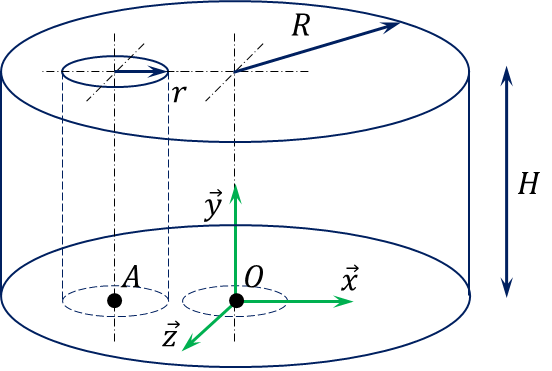
\includegraphics[width=\linewidth]{43_01}
\end{marginfigure}
\fi


\question{Déterminer la position du centre d'inertie $G$ du solide.}
\ifprof
\else
\fi

\question{Déterminer la matrice d'inertie du solide en $G$ puis en $O$.}
\ifprof ~\\
\else
\fi


\ifprof
\else
\marginnote{Corrigé voir \ref{DYN:03:B2:10:43}.}
\fi